% ---------------------------------------------------------------------------------------
\chapter{Coficientes para la comparaci\'on entre dos imagenes}\label{chap3}

En este cap\'itulo discutiremos distintos m\'etodos para realizar comparaciones entre imagenes. Notemos que dado que nuestro objetivo final es comprar una imagen con su transformada de Box y Cox, 



\section[]{Correlaci\'on de Pearson}

\subsection{Discucion sobre el coef.}

	donde se publico, como su ocupa, despcion en palabras
 
\section{Definiciones}

El coef. se define como:
\begin{equation}\label{pearson_orig}
	\rho_{X,Y}=\frac{cov(X,Y)}{\sigma_X\sigma_Y}
\end{equation}

Para una muestra de tama\~no $N$, tenemos:

\begin{equation}\label{pearson_r}
	r=\frac{\sum_{i}^N\left(x_{i}-\bar{x}\right)\left(y_{i}-\bar{y}\right)}{\sqrt{\sum_{i}^n\left(x_{i}-\bar{x}\right)^{2}} \sqrt{\sum_{i}^n\left(y_{i}-\bar{y}\right)^{2}}}
\end{equation}

Con $x_i,y_i$ elementos de la muestra y $\bar{x},\bar{y}$ sus respectivos promedios.

Hablar de The Ineffectiveness of the Correlation Coefficient for Image Comparisons

\newpage
\section[]{\textit{Maximal Information Coeficient}}
%Reshef.SOM.v2.pdf

\subsection{Sobre el coeficiente}

	El coeficiente de informaci\'on m\'axima (Maximal Information Coefficient o MIC) es una medida estad\'istica propuesta por Reshef et al. en su paper "Detecting Novel Associations in Large Data Sets" [citar]. Este coeficiente mide la correlaci\'on entre dos variables en un conjunto de datos y se basa en la idea de que una relaci\'on fuerte entre dos variables deber\'ia ser capaz de predecir una variable a partir de la otra de manera precisa.

	En su paper, Reshef et al. presentan un enfoque innovador para detectar asociaciones nobles en grandes conjuntos de datos, en lugar de buscar correlaciones fuertes entre dos variables, el coeficiente MIC permite detectar relaciones d\'ebiles pero a\'un importantes que pueden no ser evidentes al simplemente mirar los datos. Esto es posible gracias a que el coeficiente MIC es capaz de capturar no solo la fuerza de la correlaci\'on entre dos variables, sino tambi\'en su precisi\'on.

	Para calcular el coeficiente, se parte de la idea de que la informaci\'on mutua entre dos variables es una medida de la precisi\'on con la que se puede predecir una variable a partir de la otra. Por lo tanto, el coeficiente se calcula como la informaci\'on mutua m\'axima posible entre dos variables, dado un conjunto de datos. Esto se hace a trav\'es de un procedimiento iterativo en el que se prueban diferentes particiones de los datos en conjuntos de entrenamiento y prueba, y se selecciona aquella que maximiza la informaci\'on mutua.

	El la siguiente secci\'on estudiaremos las definiciones que nos entrega cada coeficiente.
 
\subsection{Definiciones}

	Como mencionamos en la parte anterior, debemos primero encontrar la informaci\'on mutua entre las variables, para esto definamos:

	\begin{defn}[Informaci\'on mutua]
		Para dos variables aleatorias conjuntas $X$ e $Y$, se define la informaci\'on mutua como:
		$$
		\mathrm{I}(X ; Y)=\int_{\mathcal{Y}} \int_{\mathcal{X}} P_{(X, Y)}(x, y) \log \left(\frac{P_{(X, Y)}(x, y)}{P_{X}(x) P_{Y}(y)}\right)dxdy
		$$
		Donde $P_{(X, Y)}$ es la funci\'on de densidad de probabilidad conjunta y $P_{X}$, $P_{Y}$, las distribuciones marginales de $X$ e $Y$ respectivamente. 
	\end{defn}

	Luego, sea $D$ un conjunto finito de pares ordenados, podemos particionar los valores de la primera coordenada en $x$ contenedores, y los valores de la segunda en $y$ de estos. Dado una malla $G$, sea $D|_G$ la distribuci\'on inducida pokr los puntos de $D$ en las celdas de $G$, i.e., la distribuci\'on en las celdas de $G$ obtenida al dejar que la funci\'on de densidad de probabilidad en cada celda sea la fracci\'on de puntos de $D$ que caen en esa celda. Veamos un ejemplo
	\begin{figure}[H]
		\centering
		\includegraphics*[scale = 0.4]{D_G_example1.png}
		\caption{Malla G de 4x3 sobre el conjunto de pares ordenados D, figura no final}
		\label{malla_G}
	\end{figure}

	Para la figura \ref{malla_G}, la funci\'on de densidad quedar\'ia de la forma:
	\[
		f_{D|_G}(i,j) = \left\{\begin{array}{lr}
			\frac{2}{10} & \text{si } (i,j) \in \{ (1,1), (2,2), (4,2)\} \\
			\frac{1}{10}, & \text{si }(i,j) \in \{ (3,2)\}  \\
			\frac{3}{10}, & \text{si }(i,j) \in \{ (4,1)\}  \\
			0, & \text{Otro caso.}
			\end{array}\right.
	\]



	Notemos que para un $D$ fijo, aunque fijemos el grosor de la malla, la distrion de esta puede variar dependiendo de donde hagamos los cortes, por ejemplo:

	\begin{figure}[H]
		\centering
		\includegraphics*[scale = 0.4]{D_G_example2.png}
		\caption{Otra malla G de 4x3 sobre el conjunto de pares ordenados D, figura no final}
		\label{malla_G_2}
	\end{figure}

	Aqu\'i podemo ver que la funci\'on de densidad que nos entrega est\'a malla es distinta a la definida para la figura \ref{malla_G_2}. Este es un hecho que explotamos en la siguiente definici\'on: 

	\begin{defn}
		Para un conjunto finito $D\in\R^2$ y enteros positivos $i,j$, definimos:
		$$
		I^*(D,i,j)=\max I(D|_G)
		$$
		donde el m\'aximo es sobre todas las mallas $G$ con $i$ columnas y $j$ filas, con $I(D|_G)$ denot la informaci\'on mutua de $D|_G$.
	\end{defn}

	Ya teniendo este valor procedemos a definir la matriz caracteristica del conjunto $D$.

	\begin{defn}
		La matriz caracteristica $M(D)$ de un conjunto bivariado $D$ es una matriz infinita con entradas:
		$$
		M(D)_{x, y}=\frac{I^{*}(D, x, y)}{\log \min \{x, y\}}
		$$
	\end{defn}
	\begin{defn}
		El coeficiente de informaci\'on m\'axima o \textit{MIC} de un conjunto bivariado $D$ de tama\~no $n$ y una malla de tama\~no menos a $B(n)$ esta dado por:
		$$
		\operatorname{MIC}(D)=\max _{x y<B(n)}\left\{M(D)_{x, y}\right\}
		$$
		donde $\omega(1)<B(n) \leq O\left(n^{1-\varepsilon}\right)$ para alg\'un $0<\varepsilon<1$ 
	\end{defn}
	\begin{rem}
		A menos que se especifique de otra forma, al momento de trabajar con esta medida usaremos $B(n)=n^{0.6}$, que es la funci\'on que ocupan en el paper citado al principio del la secci\'on
	\end{rem}
\subsection[]{Ejemplos}

	Ya con la funci\'on bien definida, veamos unos ejemplos del coeficiente, primero para algunos datos, y luego entre im\'agenes. Comenzemos por algunos ejemplos usando 

	el formato de esta secci\'on es temporal

	\begin{figure}[H]
		\centering
		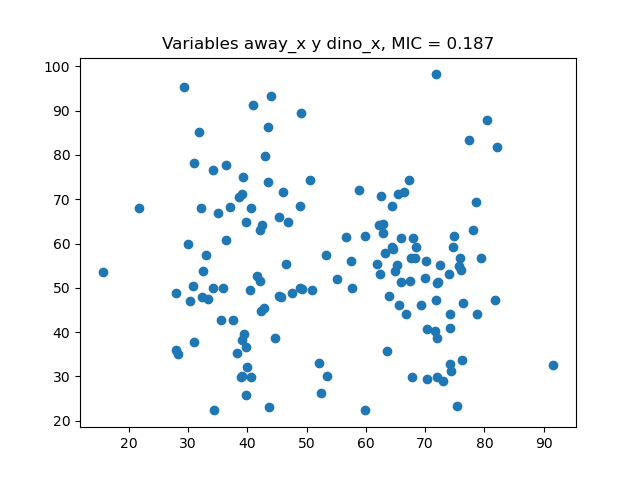
\includegraphics[scale=0.6]{away_x_dino_x_.png}
		\caption{ MIC = 0.187}
		\end{figure}
		
		\begin{figure}[H]
		\centering
		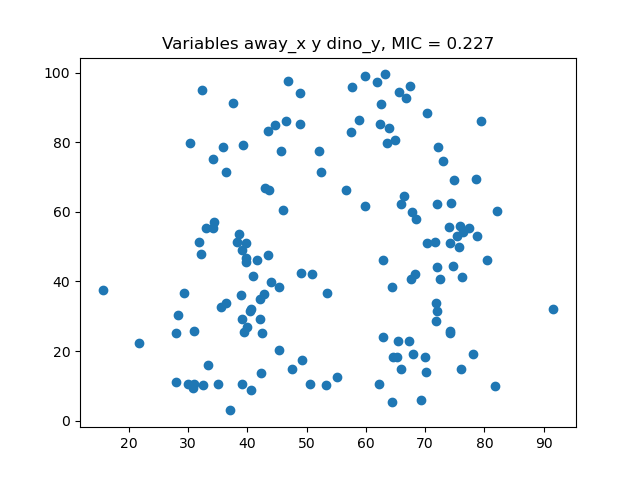
\includegraphics[scale=0.6]{away_x_dino_y_.png}
		\caption{ MIC = 0.227}
		\end{figure}
		
		\begin{figure}[H]
		\centering
		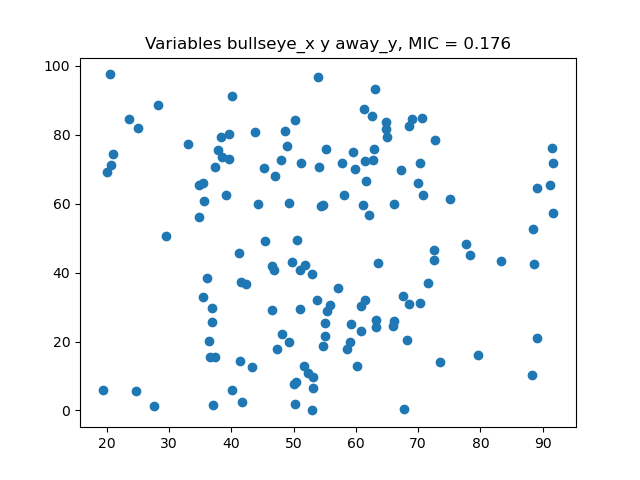
\includegraphics[scale=0.6]{bullseye_x_away_y_.png}
		\caption{ MIC = 0.176}
		\end{figure}
		
		\begin{figure}[H]
		\centering
		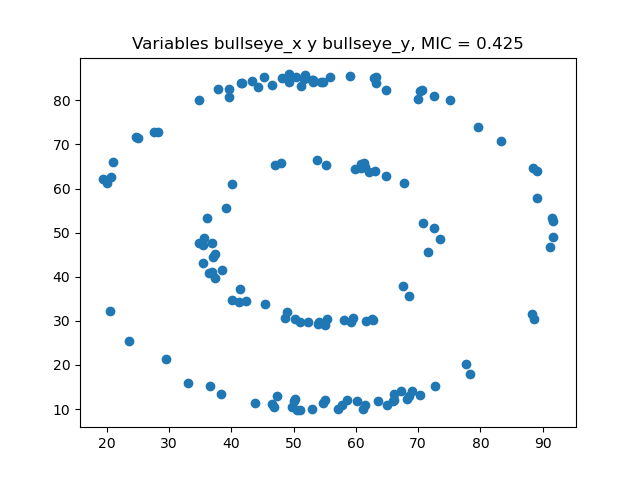
\includegraphics[scale=0.6]{bullseye_x_bullseye_y_.png}
		\caption{ MIC = 0.425}
		\end{figure}
		
		\begin{figure}[H]
		\centering
		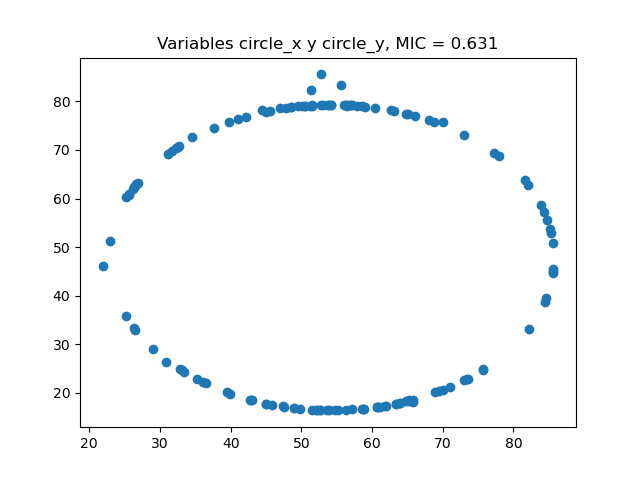
\includegraphics[scale=0.6]{circle_x_circle_y_.png}
		\caption{ MIC = 0.631}
		\end{figure}
		
		\begin{figure}[H]
		\centering
		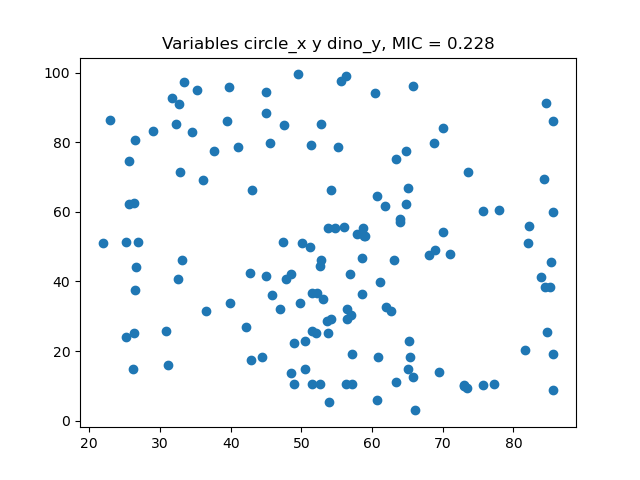
\includegraphics[scale=0.6]{circle_x_dino_y_.png}
		\caption{ MIC = 0.228}
		\end{figure}
		
		\begin{figure}[H]
		\centering
		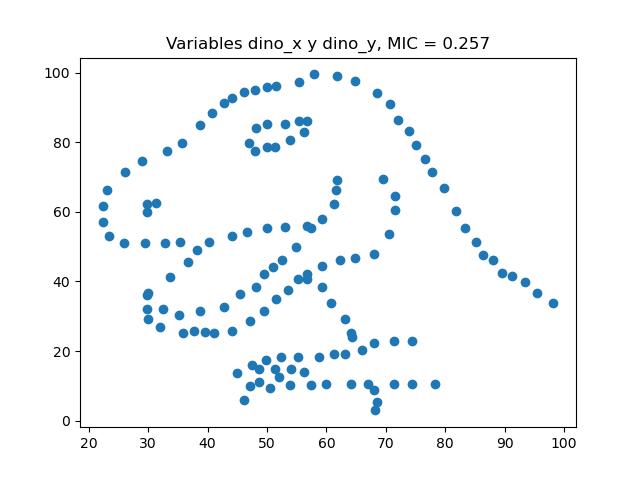
\includegraphics[scale=0.6]{dino_x_dino_y_.png}
		\caption{ MIC = 0.257}
		\end{figure}
		
		\begin{figure}[H]
		\centering
		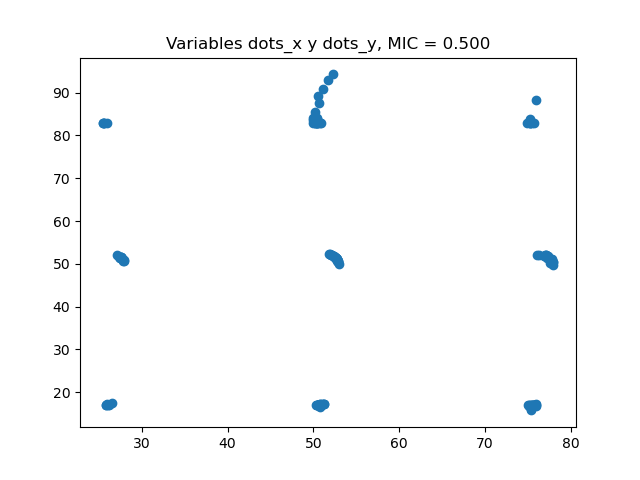
\includegraphics[scale=0.6]{dots_x_dots_y_.png}
		\caption{ MIC = 0.500}
		\end{figure}
		
		\begin{figure}[H]
		\centering
		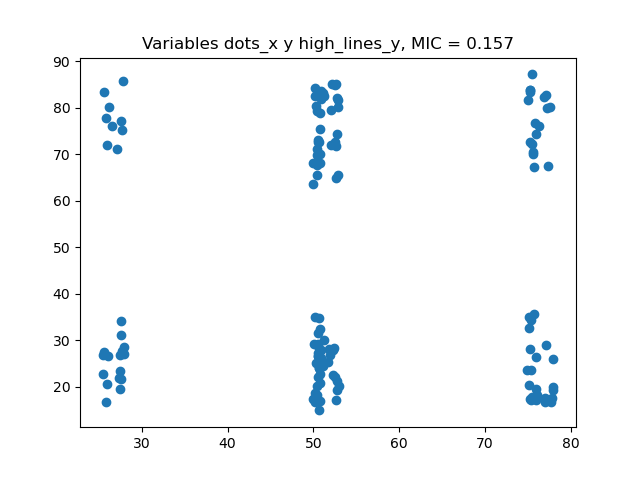
\includegraphics[scale=0.6]{dots_x_high_lines_y_.png}
		\caption{ MIC = 0.157}
		\end{figure}
		
		\begin{figure}[H]
		\centering
		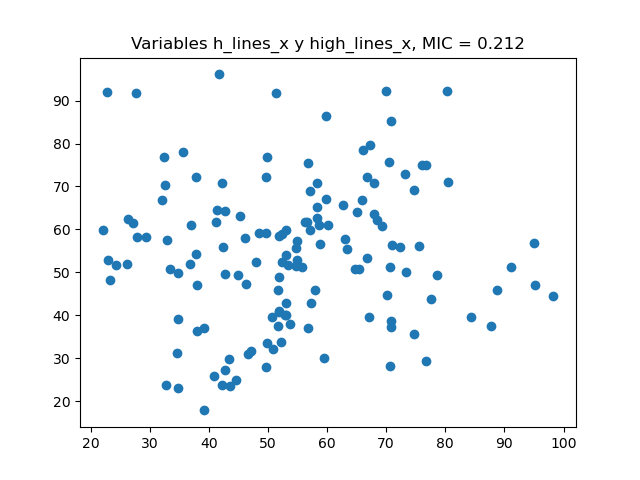
\includegraphics[scale=0.6]{h_lines_x_high_lines_x_.png}
		\caption{ MIC = 0.212}
		\end{figure}
		\subsection{Hablar sobre el algoritmo y el papaer del 2016, que es TICe y MICe}

\newpage

	\subsection{Hablar sobre el algoritmo y el papaer del 2016, que es TICe y MICe}

\section[]{Correlaci\'on local} 

	%chen2010.pdf

	\subsection{Discucion sobre el coef.}

	donde se publico, como su ocupa, despcion en palabras

	La correlaci\'on local, tamb\'ien conodica como coeficiente no param\'etrico de Chen, o coeficiente de Chen. Este, sin realizar supuestos sobre distribuciones, detecta relaciones no lineales al invenstigar un mont\'on de correalciones locales. 

	\subsection{Definiciones}

	La definici\'on del m\'etodo est\'a basada en en el concepto de integrales de correlaci\'on, las cuales se definen de la siguiente forma:
	\begin{defn}
		$$
		I(r)=\lim _{N \rightarrow \infty}\left\{\frac{1}{N^{2}} \sum_{i, j=1}^{N} I\left(\left|z_{i}-z_{j}\right|<r\right)\right\}
		$$
	\end{defn}
	La integral de correlaci\'on cuantifica el el n\'umero promedio de vecinos dentro de un radio $r$. Notemos que esta definici\'on sigue teniendo sentido cuando los datos no son series de tiempo.

	Para desarrollar una medida de asociaci\'on entre vectores, $x$ e $y$, modificamos la definici\'on de $I(r)$ como sigue. Sean $z_i=(x_i,y_i)$ con $i=1,\dots, N$ las observaciones en el conjunto de datos. Sea $|z_i-z_j|$ la distancia euclidiana. Definimos $\hat{I}(r)=\frac{1}{N^{2}} \sum_{i, j=1}^{N} I\left(\left|z_{i}-z_{j}\right|<r\right)$. Las distancias obsevadas son adem\'as linealmente transformadas para que se encuentren entres 0 y 1 antes de calcular $\hat{I}$. Notemos que $\hat{I}$a tiene las propiedades de una funci\'on de distribuci\'on acumulativa. Es no decreciente entre 0 y 1 y continua por la derecha. La funci\'on $\hat{I}(r)$ descrive el patr\'on global de distancias entre vecinos. 

	Nuestro inter\'es principal es la definici\'on  de una metrica para cuantificar la asosiaci\'on no lineal estudiando patrones locale. Dado esto, definimos la densidad de vecinos $D$ de forma similar a la derivada de $\hat{I}$: 

	$$
		\hat{D}(r)= \frac{\vartriangle\hat{I}(r)}{\vartriangle r}
	$$

	Donde $\vartriangle\hat{I}(r)$ denota un cambio en $\hat{I}(r)$. La densidad de vecinos es evaluada en radio distreto r, con $r=0,1/m, 2/m, \dots, 1$  y $m$ es un grosor de malla arbitrario. Una funci\'on de suavizado autom\'atico usando validaci\'on cruzada es usada para elegir un \'optimo el tama\~no $m$ (Vilela et al. 2007) y se aplica para suavizar $D(r)$. En el paper, el tama\~no predeterminado $m$ se establece como $N$, el n\'umero de observaciones y en este trabajo usaremos el mismo $m$. El estad\'istico $\hat{D}$ es una aproximaci\'on discreta de $d\hat{I}(r)/d r$, la cual tiene las propiedades formales de una probabilidad funci\'on de densidad. Por lo tanto, con un ligero abuso de terminolog\'ia nos referimos a $\widehat{D}(r)$ como una distribuci\'on.

	En base a esto definimos la correlaci\'on local. Intuitivamente, las distancias entre los puntos de datos entre dos variables correlacionadas diferir\'ian de las distancias entre dos variables no correlacionadas. Sea $\widehat{D_0}(r)$ la estimaci\'on de una distribuci\'on nula, que se compone de dos vectores sin asociaci\'on. Definimos la correlaci\'on local ($\ell(r)$) como la desviaci\'on de D de la de la distribuci\'on nula a una distancia vecina dada r:

	$$
		\ell(r)=\widehat{D}(r)-\widehat{D}_{0}(r)
	$$

	Este enfoque no asume ninguna distribuci\'on param\'etrica. La flexibilidad de este m\'etodo facilita el cambio de la distribuci\'on nula a cualquier distribuci\'on de inter\'es. 
	
	Por ultimo, definimos el coficiente como de correlaci\'on local m\'axima, o coeficiente de Chen como:
	$$
		M=\max _{r}\{|\ell(r)|\}
	$$
	La interpretaci\'on de $\ell(r)$ como la diferencia de dos distribuciones implica que $M$ puede interpretarse como la distancia bajo la norma del supremo entre $\widehat{D}$ y $\widehat{D_0}$. En otras palabras, definimos el estad\'istico M como la desviaci\'on m\'axima entre dos densidades vecinas subyacentes.